\section{Patrons Retenus}

\subsection{Builder et Decorator}

\begin{figure}[!ht]
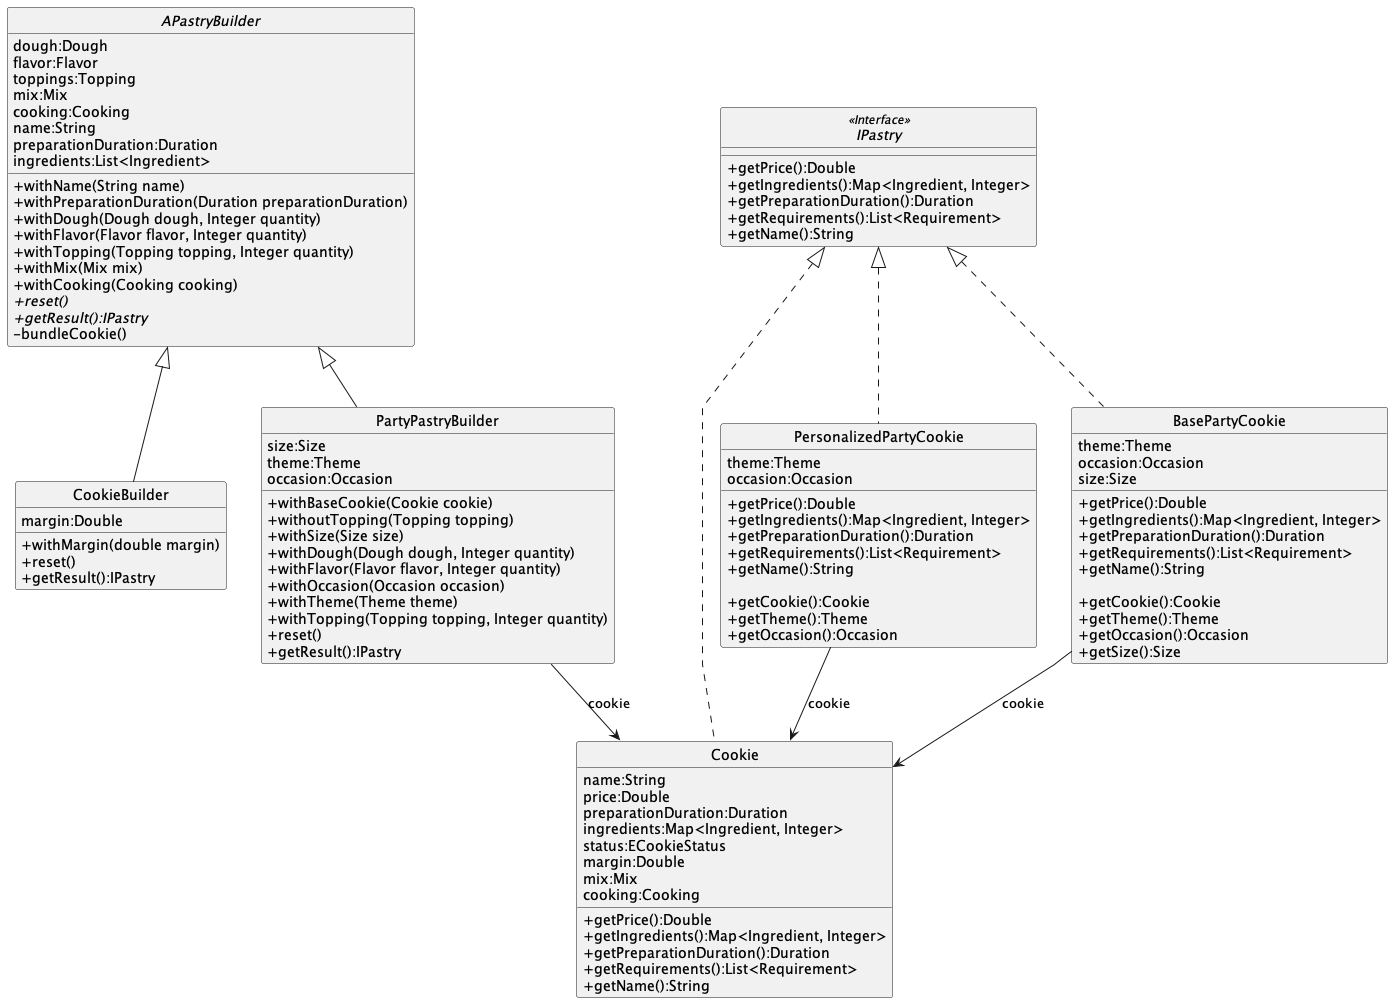
\includegraphics[width=1\textwidth]{builderDecoratorPattern}
\centering
\caption{Diagramme de Classe simplifié des Patrons Builder et Decorator}
\label{uml:builder-decorator}
\end{figure}

\paragraph{Builder: } nous avons choisi 
d'utiliser ce patron de conception à deux reprises dans notre application.
Dans un premier temps, nous l'avons utilisé pour la création de nouvelles recettes.
En effet, lorsque nous souhaitons créer une recette de cookie, il est entre autre nécessaire 
de renseigner un nom, une liste d'ingrédients, un prix, un type de cuisson, etc.
Pour mettre en place ce patron de conception, nous avons créé la classe CookieBuilder qui expose des 
méthodes tel que withName, withFlavor, getResult. 
Son utilisation nous permet de faciliter création des recettes en choisissant les attribut que 
nous souhaitons initialiser et en gardant dans attribut par défauts pour ceux qui ne sont pas définis.

\paragraph{Decorator: } dans un second temps, nous avons associé les patrons de conception Builder et Decorator
pour la création de cookies festif (PartyCookies). Le patron de conception Decorator nous permet 
de modifier les caractéristiques d'un cookie de base (prix, taille, ingrédients, durée de préparation) ainsi que d'ajouter 
de nouveaux attributs (thème, occasion, ...), sans avoir à modifier la classe Cookie. 
Son association avec le Builder nous permet d'abstraire le choix du type de PartyCookie qui sera créé.
Nous pouvons donc obtenir a la fin du processus de création un cookie de type PersonalizedPartyCookie, qui est un cookie entièrement personnalisé,
ou un cookie de type BasePartyCookie qui est un cookie standard dont la taille a été augmentée.
Le choix du type de cookie dépendra uniquement des éléments qui ont été ajouté lors de la création du cookie par le PartyCookieBuilder.


\subsection{Observer}

\begin{figure}[!ht]
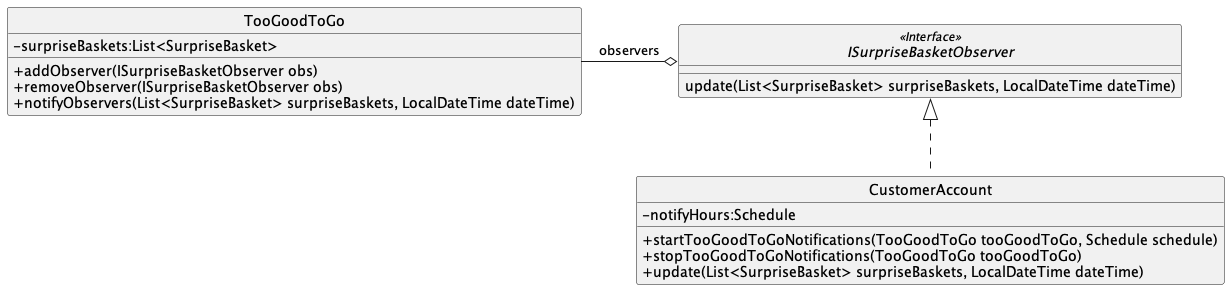
\includegraphics[width=1\textwidth]{observerPattern}
\centering
\caption{Diagramme de Classe simplifié du Patron Observer}
\label{uml:observer}
\end{figure}


\paragraph{Observer: } pour mettre en place le service TooGoodToGo dans notre application,
nous avons choisi d'utiliser le patron de conception Observer. Les clients doivent pouvoir facilement 
s'abonner et se désabonner des notifications TooGooToGo.
Le patron de conception Observer semble bien répondre à ce cas d'utilisation. 
Chaque client peut s'inscrire aux notifications TooGoodToGo par l'intermédiaire 
de la méthode startToGoodToGoNotifications. Il est alors ajouté aux observers des paniers 
surprise et lorsqu'un nouveau panier est ajouté, tous les observers sont notifiés.
Les clients peuvent également à l'inscription au service choisir les horaires et les 
jours auxquels ils veulent être notifiés en signifiant un calendrier (schedule).


\subsection{Proxy}

\begin{figure}[!ht]
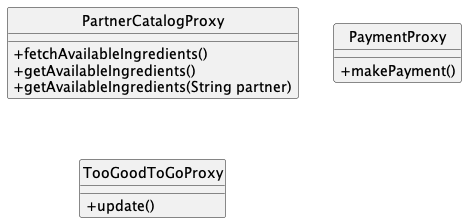
\includegraphics[width=0.5\textwidth]{proxyPattern}
\centering
\caption{Diagramme de Classe simplifié des Objets Proxy}
\label{uml:proxy}
\end{figure}

\paragraph{Proxy: } nous avons choisi d'implémenter le design pattern Proxy sur les classes
ayant pour responsabilité le dialogue avec des services partenaires comme le catalogue d'ingrédient,
le service de paiement ou l'application TooGooToGo. 
Ce patron de conception consiste à mettre en place un objet intermédiaire qui va représenter un objet distant.
Il permet entre autre de contrôler l'accès à ces objets et permet de facilement remplacer l'objet réel par un objet simulé.

\subsection{Command dans le cas de la gestion du status de la commande}

\begin{figure}[!ht]
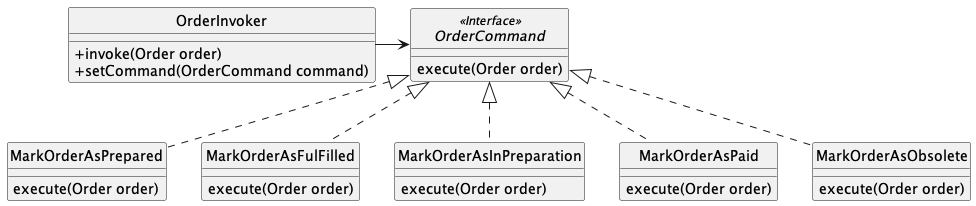
\includegraphics[width=0.8\textwidth]{commandOrderStatusPattern}
\centering
\caption{Diagramme de Classe du design pattern command dans la gestion des status de commandes}
\label{uml:proxy}
\end{figure}

\paragraph{Command: } nous avons choisi d'implémenter le design pattern Command pour gérer le changement de status de la commande,
en partant de l'idée que c'est bien fait par des invocations de la part des acteurs du système. 
Ainsi, la responsabilité de la classe 'OrderInvoker' est d'exécuter le bon algorithme de mise à jour (spécifier au démarrage dans le contexte du système) sur la bonne ressource réceptrice (le bon order). 
Ce design pattern permet d'extraire un algorithme avec ses conditions d'exécution dans une classe à part et donne la liberté de gérer les cas d'erreurs, et même d'implémenter des opération d'undo/redo, chose qu'on a pas pu l'implémenter dans le temps permis.
